

\tikzset{every picture/.style={line width=0.75pt}} %set default line width to 0.75pt        

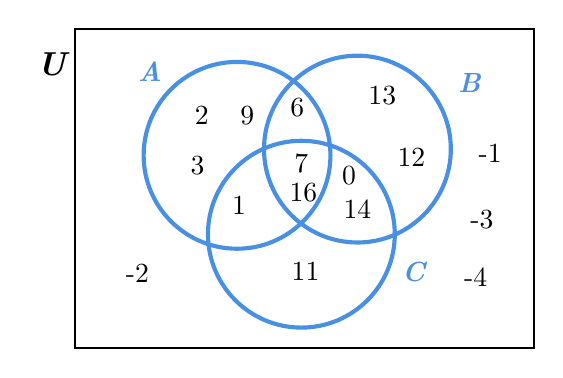
\begin{tikzpicture}[x=0.75pt,y=0.75pt,yscale=-1,xscale=1]
%uncomment if require: \path (0,174); %set diagram left start at 0, and has height of 174

%Shape: Rectangle [id:dp1682691262417073] 
\draw   (196,11) -- (417,11) -- (417,165) -- (196,165) -- cycle ;
%Shape: Circle [id:dp9745922961451678] 
\draw  [color={rgb, 255:red, 74; green, 144; blue, 226 }  ,draw opacity=1 ][line width=1.5]  (229,72) .. controls (229,47.15) and (249.15,27) .. (274,27) .. controls (298.85,27) and (319,47.15) .. (319,72) .. controls (319,96.85) and (298.85,117) .. (274,117) .. controls (249.15,117) and (229,96.85) .. (229,72) -- cycle ;
%Shape: Circle [id:dp8474368770572143] 
\draw  [color={rgb, 255:red, 74; green, 144; blue, 226 }  ,draw opacity=1 ][line width=1.5]  (287,69) .. controls (287,44.15) and (307.15,24) .. (332,24) .. controls (356.85,24) and (377,44.15) .. (377,69) .. controls (377,93.85) and (356.85,114) .. (332,114) .. controls (307.15,114) and (287,93.85) .. (287,69) -- cycle ;
%Shape: Circle [id:dp6400414490169681] 
\draw  [color={rgb, 255:red, 74; green, 144; blue, 226 }  ,draw opacity=1 ][line width=1.5]  (260,110) .. controls (260,85.15) and (280.15,65) .. (305,65) .. controls (329.85,65) and (350,85.15) .. (350,110) .. controls (350,134.85) and (329.85,155) .. (305,155) .. controls (280.15,155) and (260,134.85) .. (260,110) -- cycle ;

% Text Node
\draw (232,32) node [color={rgb, 255:red, 74; green, 144; blue, 226 }  ,opacity=1 ] [align=left] {\textbf{\textit{A}}};
% Text Node
\draw (386,37) node  [align=left] {\textbf{\textit{\textcolor[rgb]{0.29,0.56,0.89}{B}}}};
% Text Node
\draw (359,128) node  [align=left] {\textbf{\textit{\textcolor[rgb]{0.29,0.56,0.89}{C}}}};
% Text Node
\draw (257,53) node  [align=left] {2};
% Text Node
\draw (255,77) node  [align=left] {3};
% Text Node
\draw (279,53) node  [align=left] {9};
% Text Node
\draw (303,49) node  [align=left] {6};
% Text Node
\draw (275,96) node  [align=left] {1};
% Text Node
\draw (305,76) node  [align=left] {7};
% Text Node
\draw (306,90) node  [align=left] {16};
% Text Node
\draw (344,43) node  [align=left] {13};
% Text Node
\draw (358,73) node  [align=left] {12};
% Text Node
\draw (307,128) node  [align=left] {11};
% Text Node
\draw (328,82) node  [align=left] {0};
% Text Node
\draw (332,98) node  [align=left] {14};
% Text Node
\draw (396,71) node  [align=left] {\mbox{-}1};
% Text Node
\draw (226,129) node  [align=left] {\mbox{-}2};
% Text Node
\draw (389,131) node  [align=left] {\mbox{-}4};
% Text Node
\draw (392,103) node  [align=left] {\mbox{-}3};
% Text Node
\draw (186,28) node  [align=left] {\textbf{\textit{{\large U}}}};


\end{tikzpicture}